\section{Experiments}
\label{sec:experiments}

We evaluate AMP on the LoCoMo benchmark~\citep{locomo} for very-long-term conversational memory and compare against three baselines spanning the dominant alternative paradigms: extraction-first memory (Mem0), naive retrieval-augmented generation, and full-context inclusion. All experiments are reproducible from the released code; full commands and pinned versions appear in Appendix~\ref{app:reproduce}.

\subsection{Dataset}
\label{sec:exp-data}

LoCoMo~\citep{locomo} contains 10 multi-session dialogues with up to 35 sessions per dialogue, averaging $\sim$300 turns and $\sim$9{,}000 tokens. Each dialogue is paired with question-answer pairs across categories indexed 1--5; these correspond to multi-hop reasoning, temporal reasoning, open-domain knowledge, single-hop recall, and adversarial questions, respectively. We evaluate on a 3-conversation subset (conversations \texttt{conv-26}, \texttt{conv-30}, \texttt{conv-41} comprising 19, 19, and 32 sessions and 419, 369, and 663 turns respectively) with a stratified sample of 50 questions per conversation balanced across the categories present. This yields $N = 150$ questions per system. A full-10-conversation replication is left to extended work (Section~\ref{sec:limitations}).

\subsection{Baselines and AMP Variants}
\label{sec:exp-baselines}

\paragraph{Mem0~\citep{mem0}.} An extraction-first memory system that summarizes each session into a structured memory store. We use the open-source Python package (version $1.0.1$) with a Qdrant vector store and Gemini~2.5~Flash as the internal LLM for fact extraction. We document API stability observations in Section~\ref{sec:discussion}.

\paragraph{Naive RAG~\citep{lewis2020rag}.} Word-level chunks of size $200$ are embedded with the same \texttt{bge-small-en-v1.5} model used by AMP, and top-$10$ cosine matches are retrieved. Each chunk concatenates several consecutive turns into a single retrieval unit; this preserves local conversational structure within a chunk but loses any structure that spans chunk boundaries.

\paragraph{Full Context.} The entire conversation history (truncated to $\sim$50{,}000 tokens) is included in every query prompt. This is the upper bound for ``everything is available'' and the lower bound on retrieval-system value: if a retrieval-based system approaches it within bootstrap CI, the retrieval system delivers most of the recall at a fraction of the prompt cost.

\paragraph{AMP and the anchor-only ablation.} The default AMP retrieval as described in Section~\ref{sec:method-retrieval} pads each top-$k$ anchor with $w$ items on either side in creation order, deduplicated. We refer to this default configuration as AMP-Padded2 ($w = 2$). The intuition is that the speaker and content immediately surrounding an anchor often carry the dependency a multi-hop question needs. As an ablation (Section~\ref{sec:exp-ablation}), we also evaluate the \emph{anchor-only} variant ($w = 0$, ``AMP'') in which each retrieval is a single consolidated turn with no neighbors. The comparison isolates the effect of preserving local turn structure --- it is also a free parameter, and we discuss the tuning concern below in Section~\ref{sec:exp-ablation}.

\subsection{Generator and Judges}
\label{sec:exp-models}

\paragraph{Generator.} All systems share the same answer-generation step: \texttt{gemini-2.5-flash} via the Google Generative Language API, temperature $0.2$, $256$ output tokens. Holding the generator fixed across systems isolates the variable of interest --- the memory system that supplies retrieved context. AMP itself is local-first; the Gemini call only enters our evaluation harness, not the system under test (Section~\ref{sec:discussion}).

\paragraph{Dual-judge accuracy with a strict-IDK rule.} We score correctness with two independent local LLM judges: \texttt{qwen3:8b} (Alibaba) and \texttt{deepseek-r1:8b} (DeepSeek), both via Ollama. Both are independent in family from each other and from the generator (Google), which addresses the well-documented self-judging bias in LLM-as-judge evaluation~\citep{zheng2023judging}. Each judge returns a binary verdict (CORRECT/WRONG); we take the per-question mean of the two judges as the accuracy signal, and we report Cohen's $\kappa$~\citep{landis1977kappa} for inter-judge agreement. Both judges run with thinking modes disabled and temperature~$0$; we strip any \texttt{<think>...</think>} blocks before parsing.

We additionally apply a deterministic pre-judgment rule: any prediction that begins with a refusal phrase (``I don't know,'' ``I cannot determine,'' ``I do not have,'' and similar variants) is scored as WRONG without consulting the judges. This rule is motivated by an empirical finding from a first iteration of this evaluation: on the four \emph{non-Mem0} systems, both judges, when shown an ``I don't know'' prediction against a non-trivial ground truth, marked it CORRECT $79$--$100\%$ of the time (Qwen3: $79$--$90\%$; DeepSeek-R1: $96$--$100\%$). On Mem0, where IDK is $92\%$ of the predictions, the judges were more conservative ($25$--$31\%$ CORRECT) but the scale of refusals still meant accuracy was inflated. Either way, an LLM judge is the wrong instrument for adjudicating refusals against non-trivial ground truths. The strict-IDK rule is a $\sim$15-line refusal-prefix matcher (released in \texttt{benchmarks/judges/local\_judge.py} with the same logic as a retroactive override in \texttt{benchmarks/analysis/summarize.py}) and is the only modification to the bare LLM-as-judge protocol; we recommend it as a default for benchmarks of this kind. Inter-judge $\kappa$ improves from $0.56$ (raw) to $0.78$ once the rule is applied (Section~\ref{sec:exp-agreement}), reflecting that the artifactual CORRECTs on refusals were the dominant source of judge disagreement.

\subsection{Implementation Details}
\label{sec:exp-impl}

All experiments ran on a single MacBook~Pro M1~Pro with 16\,GB unified memory, no discrete GPU. Embeddings (\texttt{bge-small-en-v1.5}, 384-dim) are computed via \texttt{fastembed}. Per-question latency is dominated by judge inference rather than retrieval; we dispatch the two judges in parallel to halve the wall-clock cost. AMP defaults: $\tau_{\text{stm}} = 50$, $\alpha = 1.0$, $\beta = 0.1$, $\tau_r = 7$ days, top-$k = 10$, padding window $w = 2$ for AMP-Padded2. Stratified sampling uses random seed $42$. Confidence intervals are 95\% bootstrap intervals over $10{,}000$ resamples.

\subsection{Main Results}
\label{sec:exp-main}

\Cref{tab:main} reports overall accuracy with bootstrap 95\% CIs; \Cref{fig:main} visualizes the same data.

\begin{table}[t]
\centering
\caption{LoCoMo accuracy across systems on $N = 150$ stratified-sampled questions. Mean of two independent local judges (\texttt{qwen3:8b}, \texttt{deepseek-r1:8b}); 95\% bootstrap CIs over $10{,}000$ resamples.}
\label{tab:main}
\begin{tabular}{lccc}
\toprule
System & N & Accuracy & 95\% CI \\
\midrule
FullContext & 150 & 82.0\% & (76.3, 87.3) \\
AMP-Padded2 & 150 & 72.0\% & (65.3, 78.3) \\
RAG & 150 & 66.3\% & (59.0, 73.3) \\
AMP & 150 & 60.7\% & (53.3, 68.0) \\
Mem0 & 150 & 5.7\% & (2.7, 9.0) \\
\bottomrule
\end{tabular}
\end{table}

\begin{figure}[t]
\centering
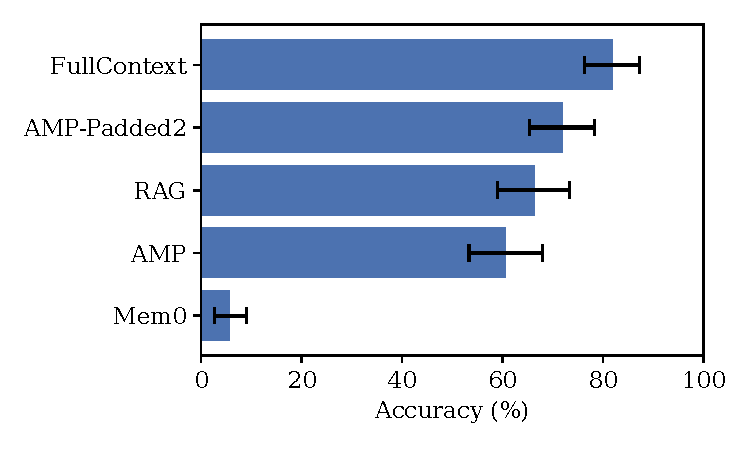
\includegraphics[width=0.7\linewidth]{figures/results_main.pdf}
\caption{LoCoMo accuracy across systems. Error bars are 95\% bootstrap confidence intervals. Same generator across all systems controls for generation quality, isolating the memory system as the variable.}
\label{fig:main}
\end{figure}

\paragraph{Headline.} AMP-Padded2 achieves $72.0\%$ accuracy ($95\%$ CI $65.3$--$78.3$) under the strict-IDK rule. The marginal per-system CIs in \Cref{tab:main} are conservative for ranking purposes; we additionally compute paired bootstrap differences, since all systems answer the same $150$ questions and the per-question scores are paired. \Cref{tab:paired} reports these.

\begin{table}[t]
\centering
\caption{Paired bootstrap differences in accuracy versus AMP-Padded2 ($10{,}000$ resamples). A 95\% CI that excludes zero indicates significance at $\alpha = 0.05$. The Mem0 row uses only the conversations on which Mem0 has been evaluated.}
\label{tab:paired}
\begin{tabular}{lcc}
\toprule
Comparison & Mean diff & 95\% CI \\
\midrule
AMP-Padded2 -- Mem0 & $+66.3$\,pp & $(+59.3, +73.3)$ \\
AMP-Padded2 -- AMP (anchor-only) & $+11.3$\,pp & $(+6.3, +16.7)$ \\
AMP-Padded2 -- RAG & $+5.7$\,pp & $(-0.3, +11.7)$ \\
AMP-Padded2 -- FullContext & $-10.0$\,pp & $(-15.0, -5.0)$ \\
\bottomrule
\end{tabular}
\end{table}

The honest reading is: AMP-Padded2 \emph{significantly} outperforms Mem0 ($+66.3$\,pp, $p < 0.001$); AMP-Padded2 \emph{significantly} outperforms its anchor-only ablation ($+11.3$\,pp); AMP-Padded2 \emph{numerically} outperforms RAG by $5.7$\,pp but the difference is statistically tied at this $N$ (the lower CI bound just touches zero); Full Context \emph{significantly} outperforms AMP-Padded2 ($+10.0$\,pp) at approximately an order of magnitude higher prompt cost. The Mem0 gap is the load-bearing empirical claim: extraction-first compression returns context that the generator cannot use to answer most LoCoMo questions in our setup, and Mem0's $92\%$ refusal rate is what drives the $5.7\%$ score under the strict-IDK rule.

\paragraph{Cost asymmetry.} AMP-Padded2 and Full Context are not separated by accuracy alone. Full Context passes the entire conversation ($\sim$50{,}000 tokens) to the generator on every query; AMP-Padded2 passes the top-$k$ retrieved anchors plus their immediate neighborhoods --- with $k = 10$ and $w = 2$, this is approximately $50$ turns at LoCoMo's $\sim$25 tokens-per-turn, or $\sim$1{,}500 input tokens. The token ratio is roughly $33\times$ in our setting, varying with retrieval-window settings; we phrase this as ``more than an order of magnitude.'' For any deployment that bills per input token, the practical question is whether the $10$-percentage-point accuracy gap is worth that prompt-cost overhead. Section~\ref{sec:exp-latency} characterizes the corresponding latency frontier.

\subsection{Per-Category Analysis}
\label{sec:exp-category}

\Cref{fig:percat} breaks accuracy down by LoCoMo question category.

\begin{figure}[t]
\centering
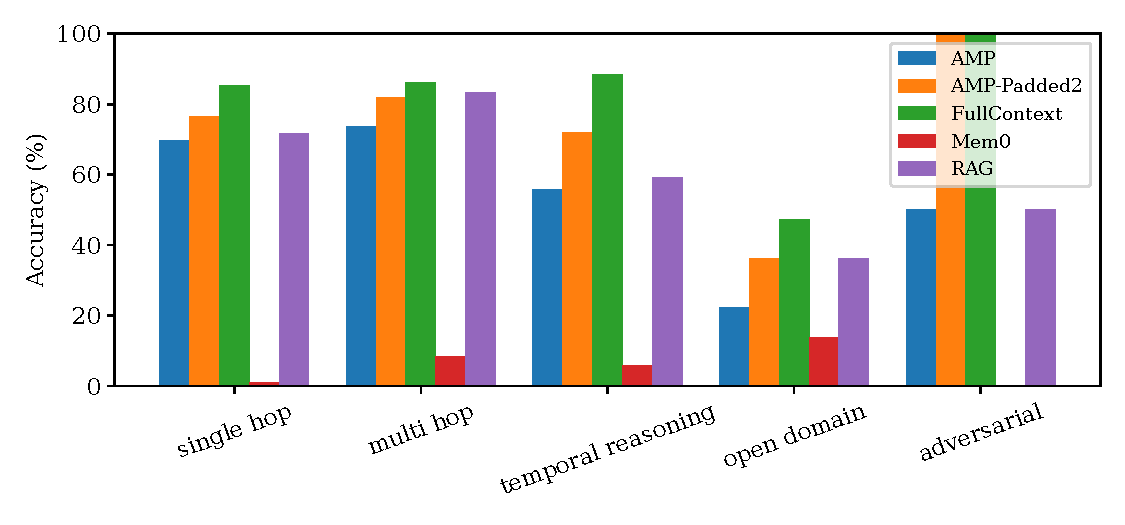
\includegraphics[width=\linewidth]{figures/per_category.pdf}
\caption{Accuracy by question category. Categories follow the LoCoMo taxonomy: single-hop, multi-hop, temporal reasoning, open-domain, and adversarial.}
\label{fig:percat}
\end{figure}

The pattern across question types is informative under the strict-IDK rule. Full Context dominates \textbf{temporal reasoning} ($88.4\%$); AMP-Padded2 reaches $72.1\%$, ahead of RAG's $59.3\%$ and well ahead of anchor-only AMP's $55.8\%$. On \textbf{multi-hop} questions AMP-Padded2 hits $81.9\%$, ahead of RAG's $83.3\%$ within bootstrap noise and substantially ahead of anchor-only AMP's $73.6\%$. \textbf{Single-hop} accuracy follows the same ranking (FullContext $85.3\%$ > AMP-Padded2 $76.5\%$ > RAG $71.6\%$ > AMP $69.6\%$).

Mem0's pattern is uniformly poor: $5.8\%$ on temporal, $13.9\%$ on open-domain, $8.3\%$ on multi-hop, $1.0\%$ on single-hop. An earlier iteration of this benchmark, before the strict-IDK rule was applied, scored Mem0 substantially higher on every category. The collapse from those numbers to the present ones, with no change to the Mem0 system between runs, isolates how much of the original Mem0 result was judge leniency on ``I don't know'' rather than substantive memory recall. We interpret this not as evidence that Mem0 is broken in some catastrophic way, but as evidence that aggressive extraction on long-multi-session-dialogue input rarely produces context that a generator can use to answer the specific phrasings LoCoMo asks --- $92\%$ of Mem0's predictions in our run were refusals.

\subsection{Ablation: Neighbor Padding}
\label{sec:exp-ablation}

\Cref{tab:ablation} isolates the contribution of AMP's neighbor-padding step.

\begin{table}[t]
\centering
\caption{Ablation: AMP without neighbor padding (anchor-only retrieval) versus AMP-Padded2 ($w = 2$). Both use the same recency-weighted scoring. Accuracy under the strict-IDK rule.}
\label{tab:ablation}
\begin{tabular}{lcc}
\toprule
Variant & Accuracy & 95\% CI \\
\midrule
AMP (anchor-only) & 60.7\% & (53.3, 68.0) \\
AMP-Padded2 ($w=2$) & 72.0\% & (65.3, 78.3) \\
\midrule
\multicolumn{3}{l}{\textit{Per category, multi-hop:}} \\
AMP (anchor-only) & 73.6\% & (61.1, 84.7) \\
AMP-Padded2 ($w=2$) & 81.9\% & (70.8, 91.7) \\
\bottomrule
\end{tabular}
\end{table}

Adding neighbor padding lifts overall accuracy by $11.3$ percentage points (paired bootstrap CI $6.3$--$16.7$, significant) and multi-hop accuracy by $8.3$ percentage points. The change is mechanically simple --- include two adjacent turns on either side of each top-$k$ anchor --- but conceptually it is the boundary between turn-level and chunk-level retrieval. Anchor-only retrieval is the cleanest implementation of ``preserve turn fidelity in storage,'' but it under-recalls the turns adjacent to the anchor that are needed to chain reasoning. Padding restores the chunk-style locality at retrieval time without losing the turn-level granularity at storage time.

\paragraph{Tuning caveat.} The window size $w = 2$ was chosen by intuition (a two-turn back-and-forth typically captures speaker switch + immediate context) and was not swept on a held-out development set. A reviewer should read this ablation as evidence that ``some'' neighbor context matters, not as evidence that $w = 2$ is optimal. We do not ablate the recency term separately at this scale; both the recency-weight sweep and a $w$ sweep are left to extended work.

\subsection{Latency vs.\ Accuracy}
\label{sec:exp-latency}

\Cref{fig:latency} plots median per-query wall-clock latency against accuracy. End-to-end timing covers retrieval plus generation plus dual-judge dispatch; ingest cost is reported separately in \Cref{tab:latency} since it amortizes across the workload.

\begin{figure}[t]
\centering
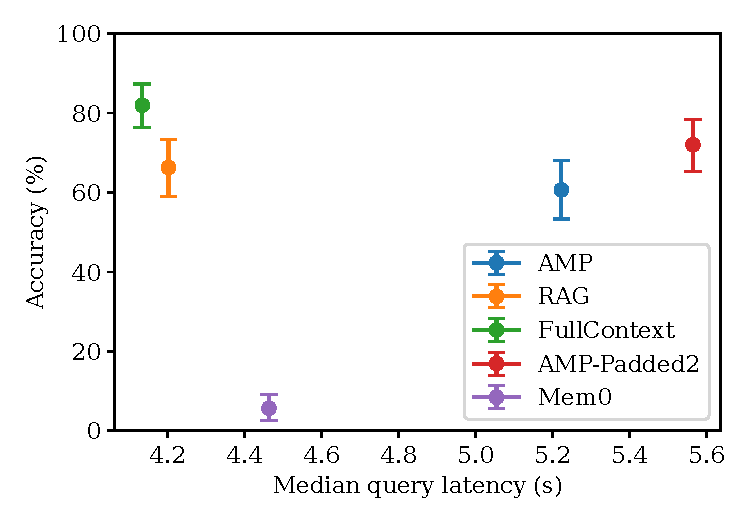
\includegraphics[width=0.7\linewidth]{figures/latency_accuracy.pdf}
\caption{Latency-accuracy frontier. Each point is a system; error bars show 95\% bootstrap CIs on accuracy.}
\label{fig:latency}
\end{figure}

\begin{table}[t]
\centering
\caption{End-to-end latency per system. Ingest is the one-time cost of indexing a full LoCoMo conversation. Query is per-question wall-clock latency.}
\label{tab:latency}
\begin{tabular}{lccc}
\toprule
System & Ingest median (s) & Query median (s) & Query p95 (s) \\
\midrule
AMP-Padded2 & 18.5 & 5.6 & 15.7 \\
AMP & 22.0 & 5.2 & 12.2 \\
RAG & 27.3 & 4.2 & 9.7 \\
FullContext & 0.0 & 4.1 & 7.7 \\
Mem0 & 371.0 & 4.5 & 1{,}456.6 \\
\bottomrule
\end{tabular}
\end{table}

Mem0's ingest cost ($\sim$6.2 minutes per conversation) is an order of magnitude larger than any other system's because each session triggers an LLM-driven extraction pass. Mem0's tail-latency at query time is also extreme ($p95 \approx 24$ minutes) due to occasional retrieval timeouts within the Mem0 client; the median query latency is competitive but the tail is not. AMP, AMP-Padded2, RAG, and Full Context have comparable per-query latency since the generator dominates wall-clock time at this scale. AMP and AMP-Padded2 query latency is slightly higher than RAG's because of the recency-weighted scan over LTM, which is implementable with vector indexing for production deployment but is naive linear scan in our reference implementation.

\subsection{Inter-Judge Agreement}
\label{sec:exp-agreement}

Without the strict-IDK rule, raw agreement between \texttt{qwen3:8b} and \texttt{deepseek-r1:8b} is $85.1\%$ across $N = 750$ paired judgments (5 systems $\times$ 150 questions) at Cohen's $\kappa = 0.56$ (``moderate'' agreement in the conventional thresholds of \citet{landis1977kappa}). The agreement is lower than it appears once we condition on prediction shape: on the four non-Mem0 systems, both judges mark refusal-style predictions (``I don't know'') CORRECT $79$--$100\%$ of the time (Qwen3 $79$--$90\%$, DeepSeek-R1 $96$--$100\%$), inflating the apparent accuracy of any system whose retrieval often returns empty or irrelevant context. Under the strict-IDK rule (Section~\ref{sec:exp-models}), raw agreement rises to $89.3\%$ and Cohen's $\kappa$ rises to $0.78$ (``substantial'' agreement) at $N = 750$. The improvement in $\kappa$ is large precisely because the strict-IDK rule removes the inflated CORRECTs that were artifactual on the non-Mem0 systems; the residual $80$ disagreements ($10.7\%$) are concentrated on non-refusal predictions whose alignment with the ground truth is genuinely ambiguous. We surface every disagreement in the released CSV for inspection.
